\chapter*{Appendix}
\phantomsection
\addcontentsline{toc}{chapter}{Appendix}
\noindent\rule{\linewidth}{2pt}

\section*{Appendix A — Hospital Unregulated Baseline Run (Full Output)}

The following screenshot shows the complete unregulated pipeline output for patient James Wilson (P-007), including the final diagnosis issued by the Chief Medical Officer with no cryptographic accountability.

This unregulated run represents the \textit{before} state — the baseline multi-agent system operating without any Attestix security layer. None of the agents hold a verifiable identity (DID/UAIT), no delegation tokens are checked before data access, no compliance profiles are validated, and no provenance entries are written. The final ruling is produced by the Chief Medical Officer agent, but there is no cryptographic link between the decision and the agent that issued it. In a real deployment, this means the decision could be tampered with retroactively, an unauthorised agent could impersonate the CMO, and there would be no audit record for a regulatory inspection. Compare this output directly against Figure~\ref{fig:carbon_result} (regulated run, same patient) to see the difference that Attestix introduces at each phase transition.

\begin{figure}[H]
\centering
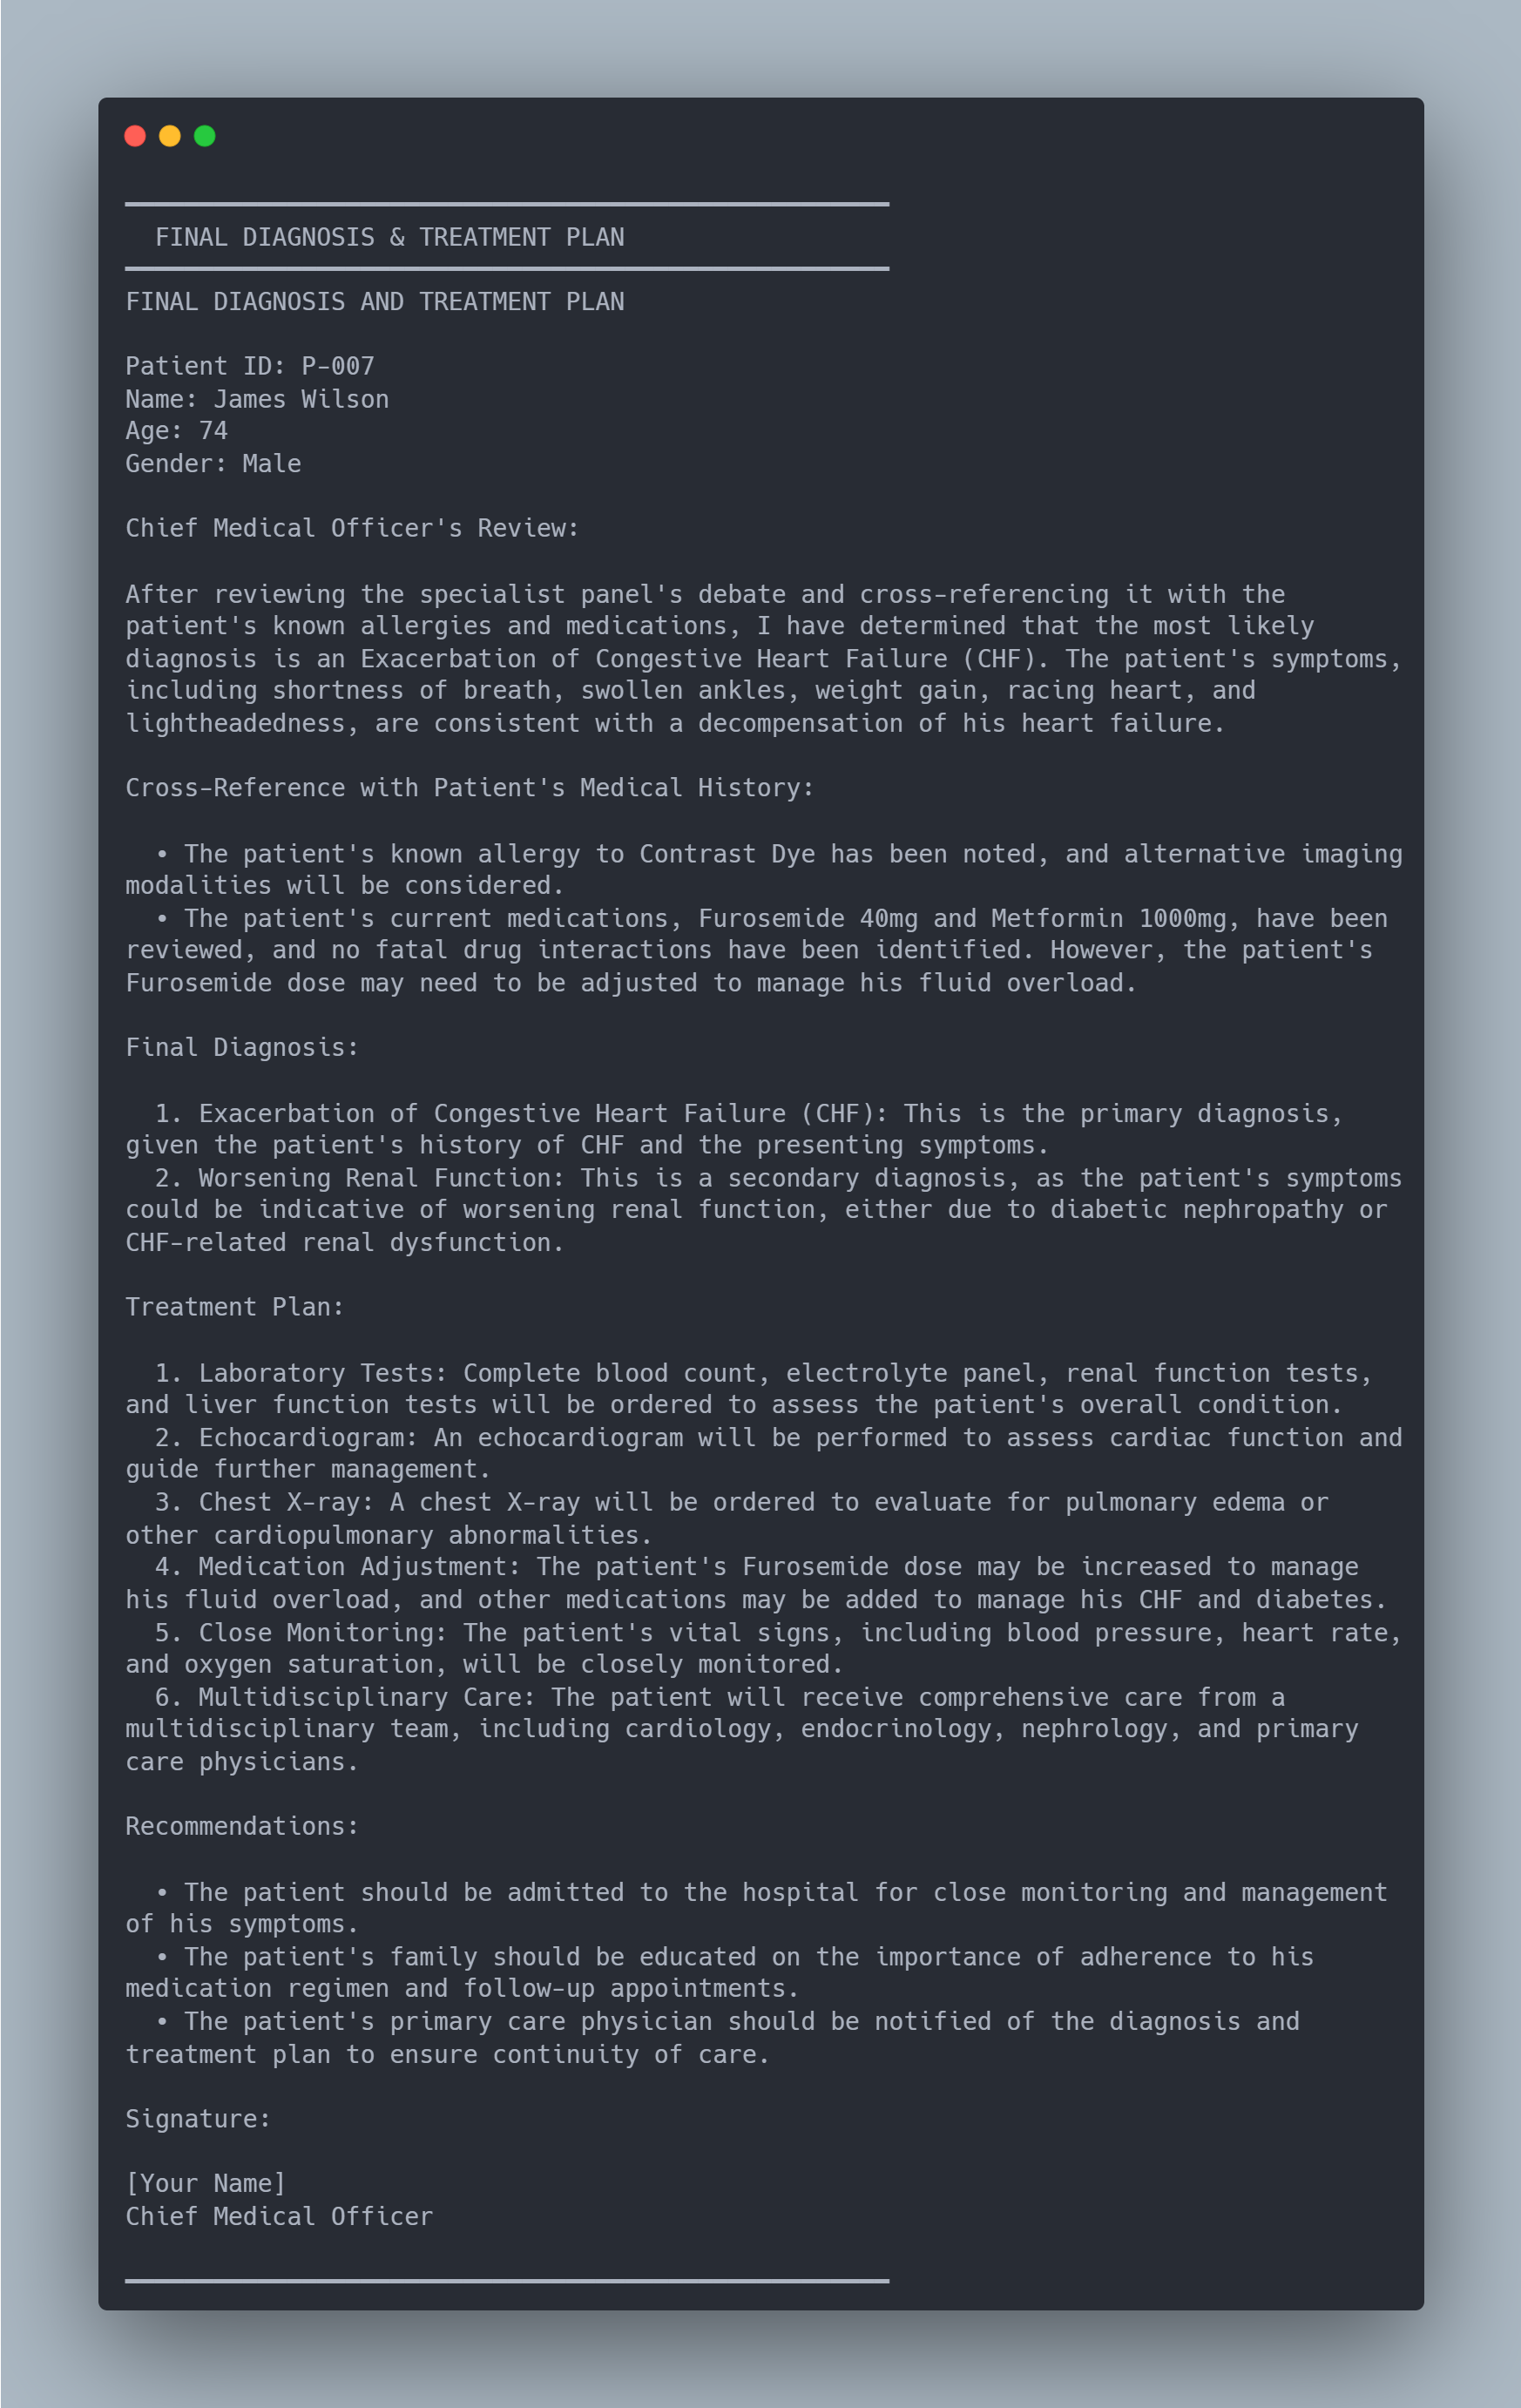
\includegraphics[width=0.88\textwidth]{carbon_before_p2.png}
\caption{Unregulated run: final diagnosis output. No audit log, no identity binding, no delegation record. The decision cannot be attributed to any specific agent after the fact.}
\label{fig:carbon_before_p2}
\end{figure}

\newpage

\section*{Appendix B — Raw Provenance Log: P-007 Hospital Run}

The following screenshots show the raw entries from \texttt{\textasciitilde/.attestix/provenance.json} for the P-007 hospital run (lines 990--1045). Each entry contains the Ed25519 signature, UCAN delegation token reference, SHA-256 chain hash, and agent DID — confirming that the cryptographic artifacts exist on disk and match the audit trail displayed in the terminal.

\begin{figure}[H]
\centering
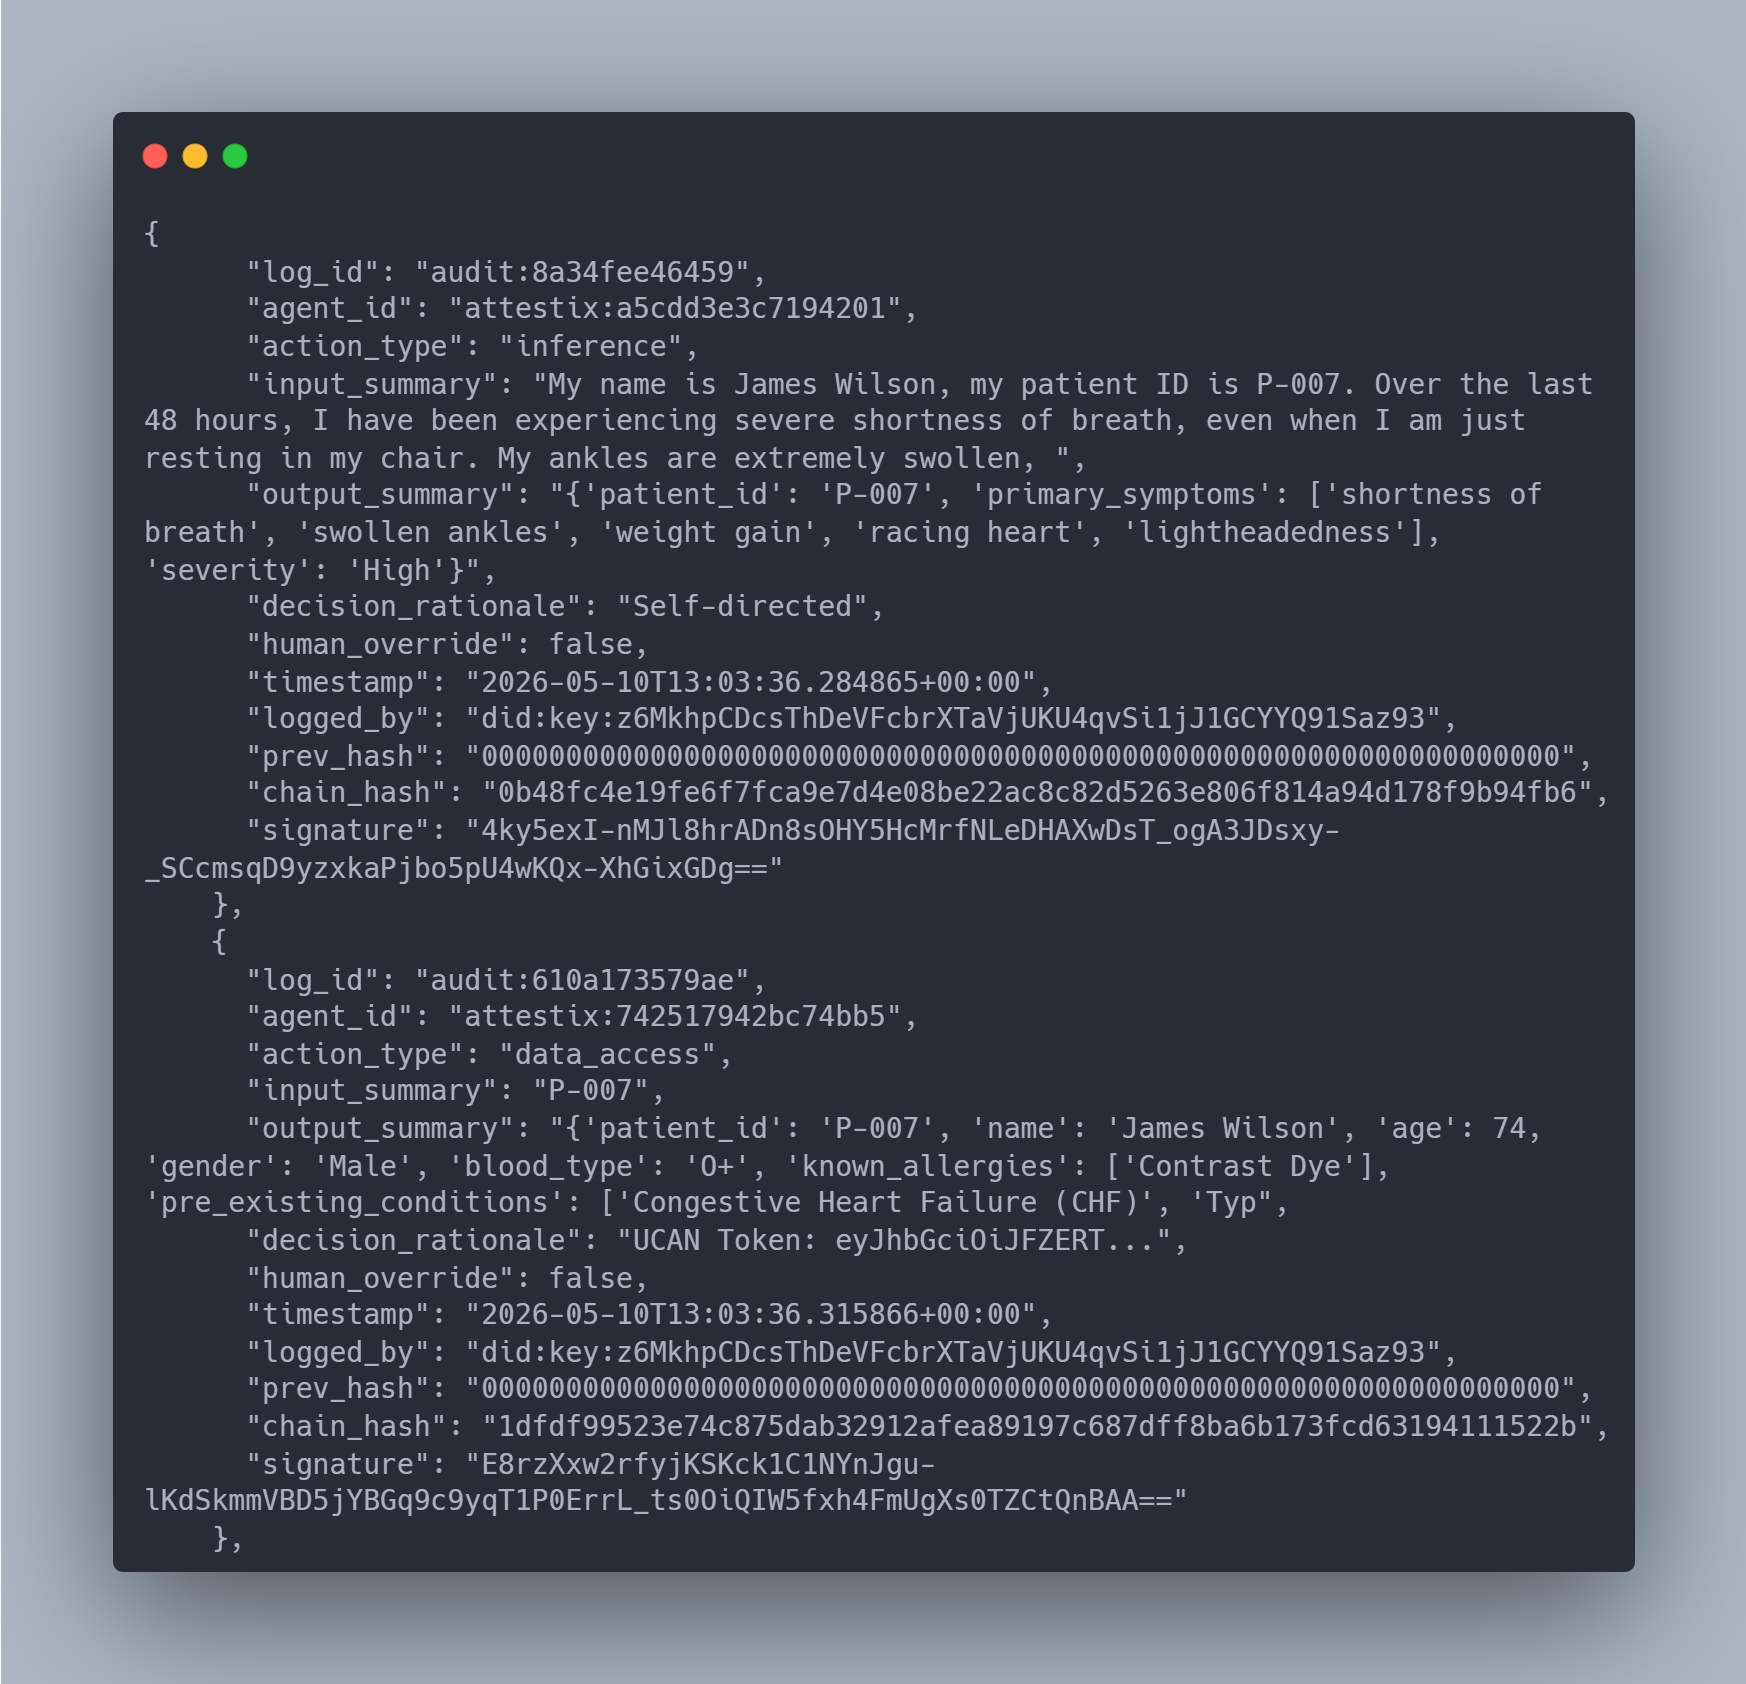
\includegraphics[width=0.88\textwidth]{carbon_provenance_p1.png}
\caption{provenance.json entries for Patient Intake Node (audit:8a34fee46459, action: inference) and Enterprise DB Node (audit:610a173579ae, action: data\_access). Both entries contain the UCAN token reference and Ed25519 signature.}
\label{fig:prov_p1}
\end{figure}

\begin{figure}[H]
\centering
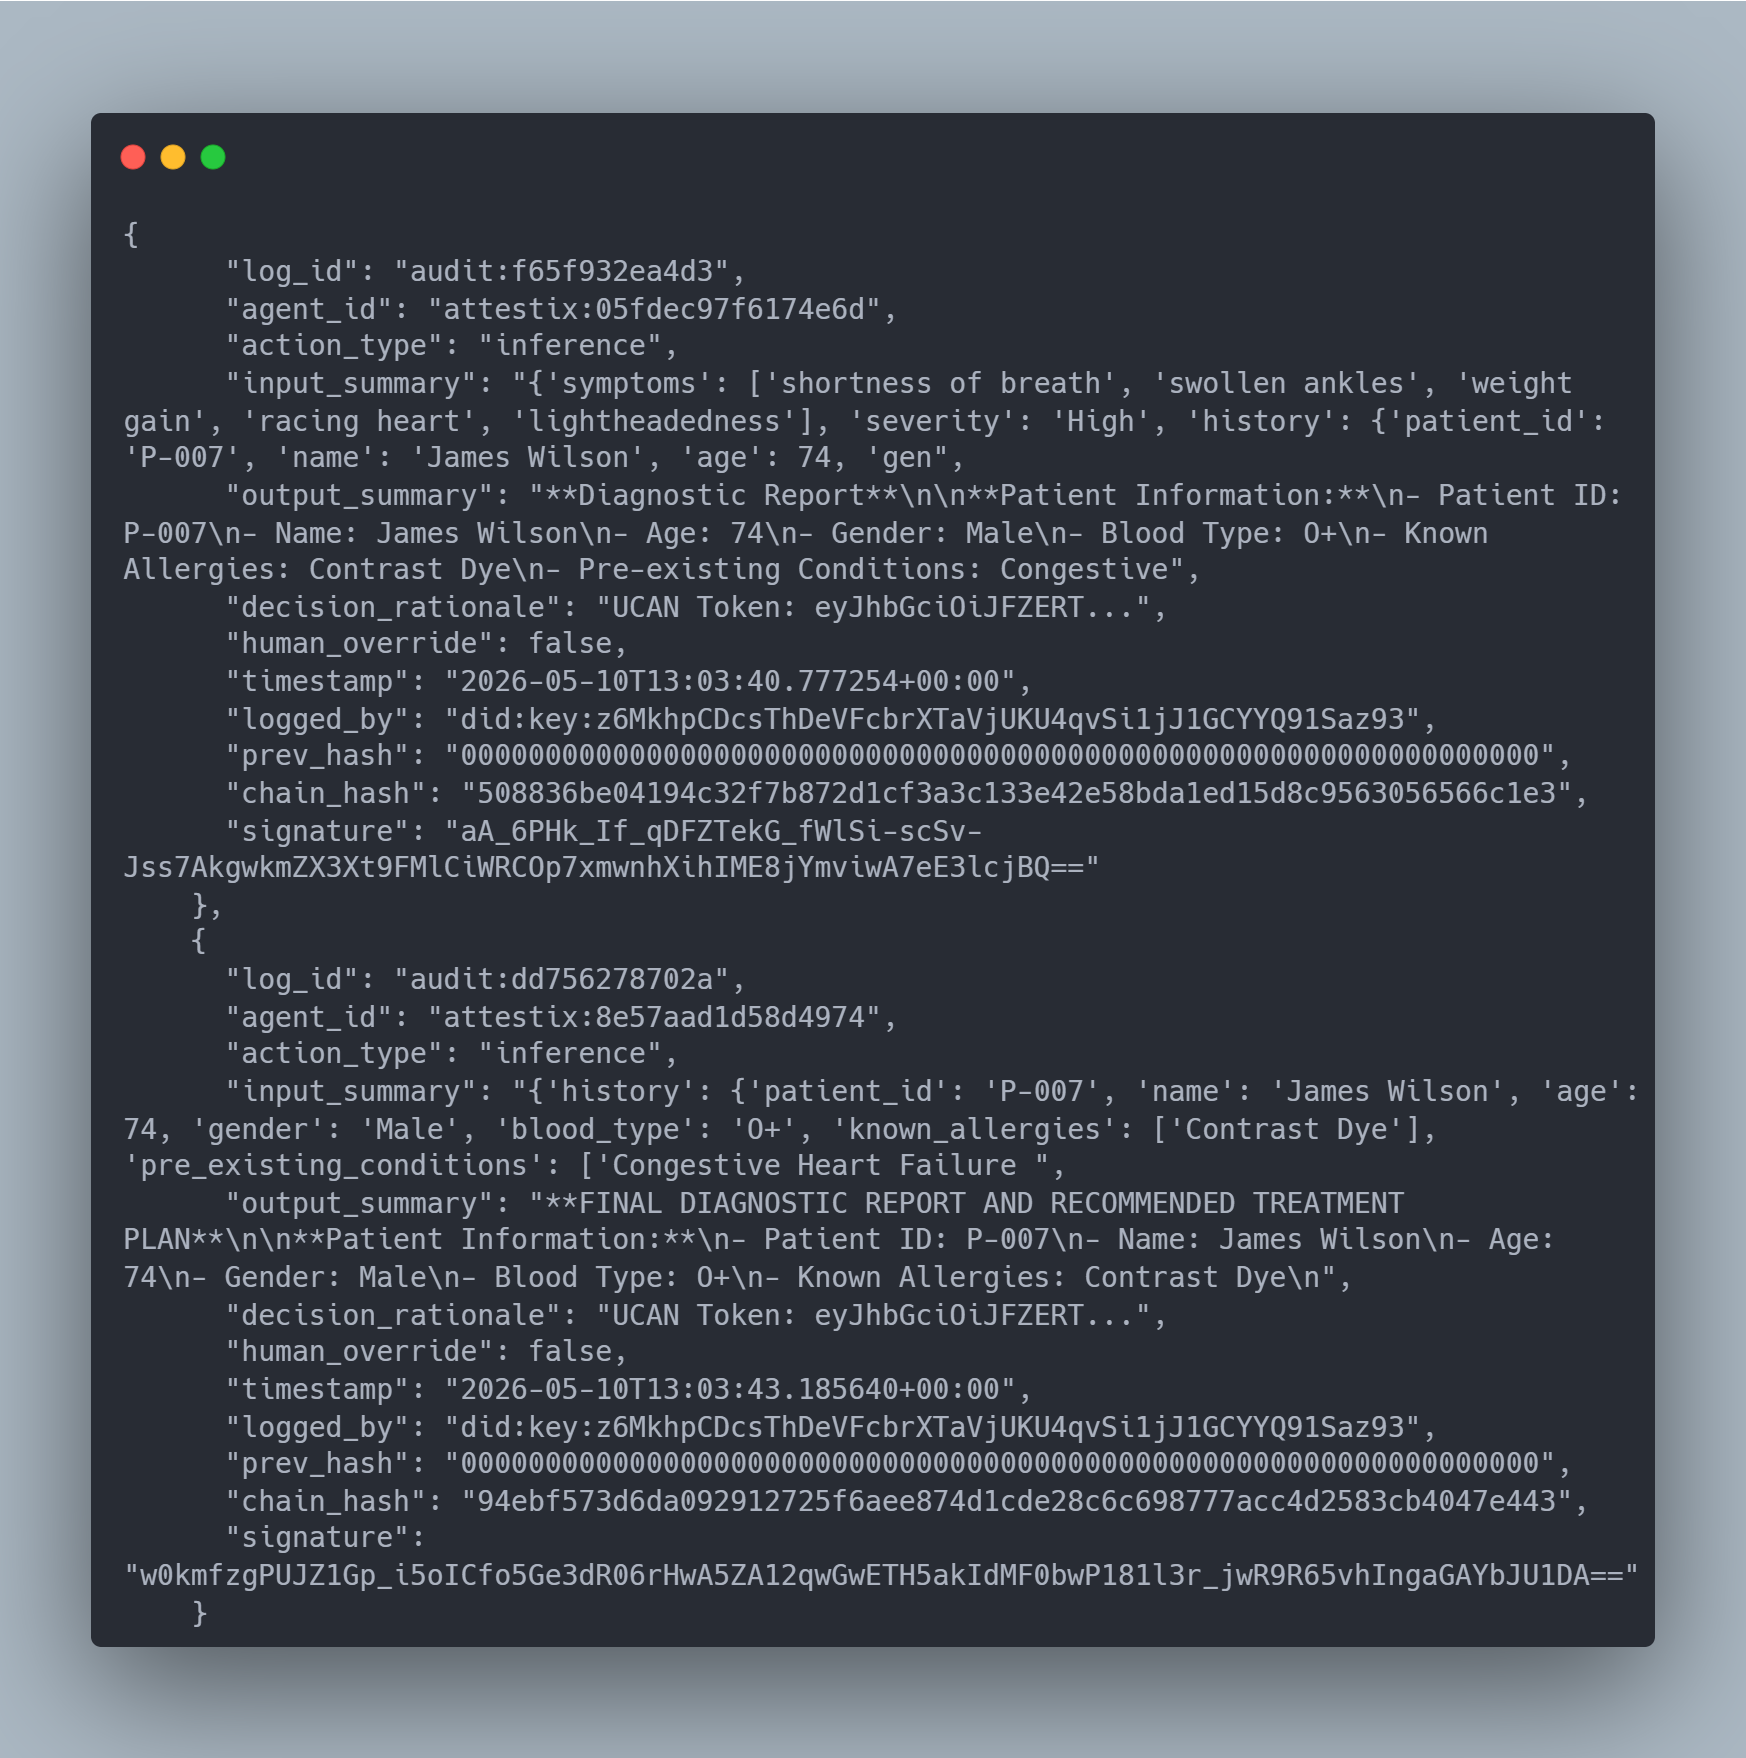
\includegraphics[width=0.88\textwidth]{carbon_provenance_p2.png}
\caption{provenance.json entries for 6-Agent Specialist Panel (audit:f65f932ea4d3, action: inference) and Chief Medical Officer (audit:dd756278702a, action: inference). All entries signed with \texttt{did:key:z6MkhpCDcs...}}
\label{fig:prov_p2}
\end{figure}

\newpage

\section*{Appendix C — Blockchain Transaction CSV Export}

The following table shows the raw CSV export from BaseScan for wallet \texttt{0xf3Fda3af...4797}, confirming all four on-chain transactions: one schema registration and three attestation attempts (two reverted due to insufficient gas, one successful).

\begin{table}[H]
\centering
\caption{BaseScan CSV Export — All Transactions for Hospital Wallet}
\begin{tabular}{|l|l|l|l|}
\hline
\textbf{TX Hash (truncated)} & \textbf{Method} & \textbf{Status} & \textbf{Block} \\
\hline
\texttt{0xdc81e16c...} & Register & Success & 41364881 \\
\texttt{0x219a603a...} & Attest & Reverted & 41364883 \\
\texttt{0xf3702424...} & Attest & Reverted & 41365207 \\
\texttt{0x107aa293...} & Attest & Success & 41365382 \\
\hline
\end{tabular}
\label{tab:csv_export}
\end{table}

\noindent The two reverted transactions confirm the gas debugging process described in Section~\ref{sec:blockchain}. The final successful transaction anchors the Merkle root permanently on Base Sepolia L2.
